\documentclass[sigconf,review,anonymous]{acmart}

\usepackage{amsmath}
\usepackage{amssymb}
\usepackage{booktabs}
\usepackage{graphicx}
\usepackage{hyperref}
\usepackage{multirow}
\usepackage{CJKutf8}                 % Chinese support for the bilingual abstract

% ACM-required dummy fields (replace at camera-ready)
\acmConference[RecSys '26]{ACM Conference on Recommender Systems}{September 2026}{Anonymous Venue}
\acmYear{2026}
\copyrightyear{2026}
\setcopyright{rightsretained}
\acmISBN{978-x-xxxx-xxxx-x/26/09}
\acmDOI{10.1145/nnnnnnn.nnnnnnn}

\settopmatter{printacmref=false}
\renewcommand\footnotetextcopyrightpermission[1]{}
\pagestyle{plain}

\begin{document}

\title{From Personalization to Statistical Discrimination: A Slice-Conditional Reranking Approach for Identity-Driven Drift in LLM-based Recommenders}

\author{Anonymous Author(s)}
\affiliation{%
  \institution{Anonymous Institution}
  \country{}}
\email{anonymous@example.com}

\renewcommand{\shortauthors}{Anonymous}

\begin{abstract}
\textbf{Background.} Large language models (LLMs) deployed as zero-shot recommenders are highly prompt-sensitive: introducing a user-identity descriptor (gender, age, race) into the prompt can shift the candidate posterior toward stereotype-aligned items, a behaviour that violates fairness criteria when it produces a measurable exposure-opportunity differential conditioned on protected attributes.
\textbf{Purpose.} We formalize this behaviour as \emph{statistical discrimination} in the sense of Dwork et al., distinct from legitimate \emph{personalization}, and propose a training-free post-hoc reranker that quantifies and mitigates the discrimination component while preserving personalization.
\textbf{Method.} Our reranker (i) builds a slice-conditional popularity matrix and applies a rank-percentile transform to recover discrimination signal under long-tail distributions, (ii) computes a per-user mainstream-ness score and adapts the rebalancing intensity $\alpha$ accordingly, and (iii) applies a top-$K'$ protection mechanism to preserve the LLM's high-confidence early ranks. We evaluate on MovieLens-1M (movie domain, $n=6{,}031$) and LastFM-1K (music track domain, $n=600$), reporting accuracy (Hit, MRR, NDCG) and exposure-fairness (APLT, Gini, Coverage, DiffScore) metrics under four demographic-conditioned scenarios.
\textbf{Findings.} On MovieLens-1M the reranker Pareto-dominates the LLM baseline, simultaneously improving NDCG (${+}8.7\%$), MRR (${+}10.7\%$), and the stereotype-defying weighted hit score (${+}12.9\%$). On LastFM-1K (track-level, long-tail-extreme) the reranker delivers a $+16$\,pp absolute APLT lift (${+}53\%$ relative) and $-10$\,pp Gini reduction, with exposure improving for $98\%$ of users and regressing for none, at the cost of $-1.6\%$ MRR and $-11\%$ NDCG. All effects are significant at $p < 10^{-5}$ in paired $t$-tests.
\textbf{Implications.} The framework provides a measurable bridge between fairness theory and operational LLM-recommender behaviour, applicable to any closed-source LLM API without retraining.
\end{abstract}

\begin{CCSXML}
<ccs2012>
   <concept>
       <concept_id>10002951.10003317.10003347</concept_id>
       <concept_desc>Information systems~Recommender systems</concept_desc>
       <concept_significance>500</concept_significance>
   </concept>
   <concept>
       <concept_id>10010147.10010178.10010187</concept_id>
       <concept_desc>Computing methodologies~Natural language generation</concept_desc>
       <concept_significance>300</concept_significance>
   </concept>
</ccs2012>
\end{CCSXML}

\ccsdesc[500]{Information systems~Recommender systems}
\ccsdesc[300]{Computing methodologies~Natural language generation}

\keywords{LLM recommendation, statistical discrimination, post-hoc reranking, popularity debias, exposure fairness, slice-conditional analysis}

\maketitle

% =================================================================
% Chinese (zh-CN) abstract — supplementary, for thesis / journal use.
% Independently composed per ARS bilingual_abstract_template guideline,
% not a mechanical translation. Disable this block for venue submission
% if Chinese abstract is not required.
% =================================================================
\begin{CJK}{UTF8}{gbsn}
\noindent\textbf{中文摘要}\medskip

\noindent\textbf{研究背景.} 大语言模型在被用作零样本推荐系统时对提示词高度敏感，当用户身份描述（性别、年龄、种族）被注入提示后，模型给出的候选分布会向语料中的刻板关联倾斜，使不同人口切片之间的物品曝光机会出现可测量的差异，从而构成对受保护特征的统计歧视。
\textbf{研究目的.} 本研究将该行为形式化为 Dwork 等人意义下的统计歧视，与合法的个性化推荐严格区分，进而提出一种无需训练的后处理重排序算法，在不降低个性化精度的前提下抑制歧视成分。
\textbf{研究方法.} 该算法包含三个关键步骤：先构建按受保护特征切片的物品流行度矩阵并施加分位数转换以在长尾数据上恢复区分信号；再利用用户历史序列计算用户在自身切片下的主流度，自适应调节重排序强度系数 $\alpha$；最后引入头部前 $K'$ 名保护机制以避免大模型的高置信首位推荐被破坏。我们在 MovieLens-1M（电影领域，6{,}031 用户）与 LastFM-1K（音乐单曲，600 用户）两个数据集上分四种人口场景同时评估准确性指标（Hit、MRR、NDCG）与曝光公平性指标（APLT、Gini、Coverage、DiffScore）。
\textbf{研究发现.} 在 MovieLens-1M 上算法相对大模型基线实现帕累托占优：NDCG 提升 8.7\%、MRR 提升 10.7\%、刻板印象加权命中分提升 12.9\%。在 LastFM-1K 单曲场景下 APLT 绝对值提升 16 个百分点（相对提升约 53\%）、Gini 下降 10 个百分点，600 用户中 98\% 的曝光得到改善而无人退化，代价为 MRR 下降 1.6\% 与 NDCG 下降 11\%；所有效应在配对 $t$ 检验下 $p < 10^{-5}$ 显著。
\textbf{研究意义.} 本工作把公平性理论与大模型推荐系统的实际行为通过可观测指标桥接起来，且无需训练即可应用于任何闭源大模型 API，为工业级部署的合规审计提供了可行路径。

\noindent\textbf{关键词:} 大模型推荐, 统计歧视, 后处理重排序, 流行度去偏, 曝光公平性, 切片条件分析, 公平性审计
\end{CJK}

\bigskip

% body sections to be added
\section{Introduction}
\label{sec:intro}

\subsection{Motivation}

Large Language Models (LLMs) are increasingly deployed as zero-shot or few-shot recommenders~\cite{liu2023chatgpt,hou2024llmranker,bao2023tallrec}. They take a natural-language prompt containing the user's interaction history and (optionally) demographic descriptors, and emit a ranked candidate list. Compared with classical collaborative filtering, LLM recommenders enjoy strong cold-start coverage, transferability across domains, and high explainability.

However, LLM recommenders inherit the statistical regularities of their pre-training corpora. When a user-identity prompt such as \emph{``the listener is a 22-year-old male''} is injected, the model's posterior over candidate items shifts in ways that reflect \textbf{the corpus's stereotyped associations} rather than purely the user's interaction history. Three failure modes are commonly observed:

\begin{itemize}
\item \textbf{Preference drift}: the model's top-ranked items change when only the demographic descriptor changes, even though the interaction history remains identical.
\item \textbf{Homogenization (category collapse)}: users sharing a demographic label receive overlapping, stereotype-aligned candidate sets, regardless of finer individual preferences.
\item \textbf{Off-category recommendation}: niche listeners under a mainstream demographic label may be served items unrelated to their actual taste, simply because those items are statistically dominant in the corpus's mental model of the demographic.
\end{itemize}

\subsection{Statistical Discrimination vs Personalization}

Following the algorithmic-fairness literature~\cite{dwork2012fairness,barocas2017fairness}, we distinguish two regimes:

\begin{itemize}
\item \textbf{Personalization.} Recommendation incrementally adapts to a user's preference signal; no systematic exposure differential is induced by protected attributes (gender, age, race) once preferences are controlled for. Legitimate; desirable.
\item \textbf{Statistical discrimination.} Recommendation systematically alters the \emph{exposure opportunity} of items conditional on a user's protected attribute, creating a measurable disparity in long-tail exposure, item coverage, or unpopularity-weighted hit rate across demographic slices. Problematic; must be mitigated.
\end{itemize}

Our framing is sharper than the colloquial \emph{``the LLM has bias''} because it ties the empirical phenomenon to a normative criterion: an LLM recommender is \textbf{discriminatory only if exposure opportunity, not just hit accuracy, differs systematically across protected demographic slices}.

\subsection{Contributions}

This paper makes four concrete contributions:

\begin{itemize}
\item \textbf{C1.} A \textbf{slice-conditional stereotype quantification} procedure (DiffScore) that scores every item by its inverse popularity within each demographic slice, and aggregates over a user's recommendation list to produce a per-(user, scenario) stereotype index that is interpretable and statistically tractable.

\item \textbf{C2.} A \textbf{user-mainstream-ness-aware adaptive reranker} that adjusts the rebalancing intensity per user: mainstream users are nudged less, niche users are protected with stronger long-tail injection. Implemented through a closed-form $\alpha$ adjustment with \emph{no training}.

\item \textbf{C3.} Two algorithmic refinements that resolve practical pathologies on long-tail-heavy datasets: (i) a \textbf{rank-percentile transformation} of the slice popularity matrix that prevents the long-tail-collapse degeneracy where the unpopularity bonus loses discrimination, and (ii) a \textbf{top-$K'$ protect} mechanism that preserves the LLM's high-confidence early-rank picks, capping MRR loss at $\leq 2\%$.

\item \textbf{C4.} \textbf{Empirical evidence on two complementary benchmarks} (ML-1M for movies; LFM-1K for music tracks). On LFM-1K our reranker delivers a $+16$\,pp absolute APLT lift (${+}53\%$ relative), $-10$\,pp Gini reduction, and net positive total weighted hit score with only $-1.6\%$ MRR. On ML-1M, the reranker achieves a Pareto-dominating outcome: NDCG and MRR both improve while exposure rebalancing also improves.
\end{itemize}

\subsection{Paper Organization}

Section~\ref{sec:related} reviews related work. Section~\ref{sec:problem} formalizes the problem. Section~\ref{sec:method} details the methodology. Section~\ref{sec:setup} describes the experimental setup. Sections~\ref{sec:results-ml1m} and~\ref{sec:results-lfm1k} present results on ML-1M and LFM-1K respectively. Section~\ref{sec:ablation} covers ablations and Pareto analysis. Section~\ref{sec:discussion} discusses limitations and future work. Section~\ref{sec:conclusion} concludes.

\section{Related Work}
\label{sec:related}

\subsection{LLM-based Recommendation}

The first wave of work on LLM recommendation focused on prompt-engineering benchmarks~\cite{liu2023chatgpt,hou2024llmranker,wang2023genrec}. Subsequent work introduced parameter-efficient fine-tuning approaches such as TALLRec~\cite{bao2023tallrec}, BIGRec~\cite{li2024bigrec}, and P5~\cite{geng2022p5}. These methods improve recommendation accuracy but do not specifically target exposure fairness. Closed-source frontier LLMs (GPT-4o, Claude-3.5, Qwen2.5) cannot be fine-tuned at all by most academic users, making post-hoc methods the only viable route in many practical settings.

\subsection{Bias and Fairness in Recommendation}

Bias in classical recommenders has been surveyed in~\cite{chen2023biassurvey}. Three intervention loci are commonly distinguished:
\begin{itemize}
\item \textbf{Pre-processing}: training-data resampling, long-tail oversampling.
\item \textbf{In-processing}: modify model architecture or loss (IPS weighting, Up5~\cite{hua2023up5}).
\item \textbf{Post-processing}: rerank model output (xQuAD~\cite{santos2010xquad}, FA*IR~\cite{zehlike2017fair}, Calibrated Recommendations~\cite{steck2018calibrated}).
\end{itemize}

For LLM recommenders specifically, recent in-processing methods include Up5~\cite{hua2023up5}, which adds fairness-aware bias tokens to a generative recommender backbone. Such methods require model fine-tuning access, which is unavailable for closed-source LLMs. The closest line to ours is post-hoc reranking on top of frozen LLM outputs; we extend it with a user-adaptive $\alpha$ and a rank-percentile $B$-transform (see Section~\ref{sec:method}).

\subsection{Stereotype Audits of LLMs}

Audits by Liu et al.~\cite{liu2023chatgpt} and Zhang et al.~\cite{zhang2024counterfactual} have demonstrated systematic preference drift in ChatGPT recommendations under identity-prompt perturbation. Our DiffScore quantification (Section~\ref{sec:method}) is directly inspired by these audits but moves beyond pure diagnosis to provide an \textbf{operational, training-free correction}.

\subsection{Long-tail and Diversity Metrics}

Abdollahpouri et al.~\cite{abdollahpouri2017aplt} introduced APLT (Average Percentage of Long-Tail items) as the standard long-tail exposure indicator. Steck~\cite{steck2018calibrated} proposed Calibration as a divergence-based diversity metric. The Gini index~\cite{atkinson1970gini} was repurposed for recommendation evaluation by Adomavicius and Kwon~\cite{adomavicius2012diversity}. We adopt all three as our exposure-fairness metrics, complementing classical accuracy metrics (Hit, Precision, Recall, MRR, NDCG).

\subsection{Position of This Work}

Our work differs from prior art on three axes:
\begin{enumerate}
\item \textbf{Framing}: we formalize the problem as \emph{statistical discrimination by exposure differential} on protected attributes, not generic ``popularity bias''. This connects empirical behaviour to fairness theory.
\item \textbf{Method}: a training-free post-hoc reranker applicable to closed-source LLMs, with novel rank-percentile $B$-transform and protect-top mechanism.
\item \textbf{Evaluation}: a paired, slice-conditional analysis with both accuracy and exposure-fairness metrics, validated across two benchmarks of distinct domain (movies, music tracks) and granularity (item-level).
\end{enumerate}

\section{Problem Formulation}
\label{sec:problem}

\subsection{Notation}

Let $\mathcal{U}$ be the user set, $\mathcal{I}$ the item catalog, and $D = \{d_1, \dots, d_p\}$ the set of protected demographic attributes. Each user $u \in \mathcal{U}$ has a feature vector $\mathbf{d}_u = (d_{u,1}, \dots, d_{u,p})$. A \emph{slice} $g$ is a value-tuple over a subset of $D$:
\begin{itemize}
\item $g = \emptyset$\,: \emph{neutral} (all users)
\item $g = \{(\textsf{gender},\textsf{male})\}$\,: \emph{gender\_M}
\item $g = \{(\textsf{gender},\textsf{female}),(\textsf{age},\textsf{young})\}$\,: \emph{cross\_F\_Youth}
\end{itemize}

Let $\mathcal{P}_u \subseteq \mathcal{I}$ denote the user's positive feedback set (items engaged at strength above threshold; see Section~\ref{sec:method}).

\subsection{Slice-Conditional Popularity}

For slice $g$ and item $i$, define the \textbf{slice-conditional positive-feedback count}:
\begin{equation}
\text{count}(i, g) = \sum_{u \in g} \mathbb{1}[i \in \mathcal{P}_u]
\end{equation}

and the \textbf{normalized slice popularity}:
\begin{equation}
B_{\text{raw}}(i, g) = \frac{\text{count}(i, g)}{\max_{j \in \mathcal{I}} \text{count}(j, g)} \in [0, 1]
\end{equation}

so that the most-engaged item per slice has $B = 1$.

\subsection{Exposure Opportunity}

Given a recommender that emits a top-$K$ list $\text{Rec}_u^{(K)}$ for user $u$, the \textbf{population-level exposure} of item $i$ is:
\begin{equation}
\text{Exp}(i) = \sum_{u \in \mathcal{U}} \mathbb{1}[i \in \text{Rec}_u^{(K)}]
\end{equation}

The \textbf{slice-conditional exposure} is:
\begin{equation}
\text{Exp}(i \mid g) = \sum_{u \in g} \mathbb{1}[i \in \text{Rec}_u^{(K)}]
\end{equation}

\subsection{Statistical Discrimination Criterion}
\label{subsec:stat-disc}

Let $f_{\text{LLM}}$ be a recommender that takes prompt features $\mathbf{x}_u = (\mathbf{h}_u, \mathbf{d}_u)$ (interaction history plus demographic descriptors) and emits $\text{Rec}_u^{(K)}$. We define $f_{\text{LLM}}$ to \textbf{statistically discriminate} if for some protected attribute $d \in D$ and pair of values $a, b$ of $d$:
\begin{equation}
\Big| \mathbb{E}_{u : d_u = a} [\Phi(\text{Rec}_u^{(K)})] - \mathbb{E}_{u : d_u = b} [\Phi(\text{Rec}_u^{(K)})] \Big| > \tau
\label{eq:stat-disc}
\end{equation}
for some exposure-related functional $\Phi$ \emph{and} the disparity is not justified by genuine within-slice preference difference.

We instantiate $\Phi$ as:
\begin{itemize}
\item $\Phi_1 = $ APLT (higher = more long-tail exposure)
\item $\Phi_2 = $ Coverage (corpus-level recommendation uniqueness)
\item $\Phi_3 = $ Gini (distributional inequality of exposure)
\end{itemize}

A reranker is \textbf{fair} in our sense if it reduces the cross-slice differential in $\Phi_1, \Phi_2, \Phi_3$ without sacrificing within-user preference alignment (measured by Hit, MRR, NDCG).

\subsection{Personalization Criterion}

A recommender preserves \emph{personalization} if, conditional on demographic attributes, the per-user list-quality metrics (MRR, NDCG, HitRate@K) do not degrade meaningfully. Our reranker targets a Pareto improvement: increase exposure fairness measurably (large effect size), decrease accuracy minimally (small effect size).

\section{Methodology}
\label{sec:method}

We split the methodology into four logical components: (\ref{subsec:preprocess}) data preprocessing, (\ref{subsec:diffscore}) slice-conditional stereotype quantification, (\ref{subsec:mainstream}) user mainstream-ness and adaptive reranking, (\ref{subsec:evalmetrics}) evaluation metrics.

\subsection{Data Preprocessing}
\label{subsec:preprocess}

\paragraph{Positive feedback definition.} A user's positive feedback is an interaction strong enough to indicate genuine preference. The exact threshold depends on dataset modality:
\begin{itemize}
\item \textbf{MovieLens-1M (ratings)}: $\text{positive}(u, i) = \mathbb{1}[r_{u,i} > 3]$.
\item \textbf{LastFM-1K (playcounts)}: $\text{positive}(u, i) = \mathbb{1}[c_{u,i} \geq 2 \land c_{u,i} > m_u]$ where $c_{u,i}$ is the play count and $m_u = \text{median}\{c_{u,j} : j \in \mathcal{I}_u\}$. The first conjunct removes one-off impressions; the second requires the play count to exceed the user's median listening intensity.
\end{itemize}

\paragraph{Train/test split.} Per-user positive items are randomly split into a training set $\mathcal{H}_u$ ($30\%$, fed as in-prompt history) and a test set $\mathcal{T}_u$ ($70\%$, withheld for evaluation):
\begin{equation}
\mathcal{T}_u = \text{Sample}_{\text{rng}}(\mathcal{P}_u, \lfloor 0.7 \cdot |\mathcal{P}_u| \rfloor), \quad \mathcal{H}_u = \mathcal{P}_u \setminus \mathcal{T}_u
\end{equation}
with a fixed seed for reproducibility.

\paragraph{Demographic slicing and sparse-slice protection.} For slices with $n_g < 30$ users, we blend with neutral:
\begin{equation}
B_{\text{blended}}(i, g) = w \cdot B_{\text{raw}}(i, g) + (1 - w) \cdot B_{\text{raw}}(i, \emptyset),\ \ w = \min(1, n_g / 30)
\end{equation}

For LFM-1K, we additionally treat \textsf{Unknown} demographic values as a first-class slice (rather than discarding users with missing fields), motivated by the fact that $71\%$ of LFM-1K users have unreported age.

\subsection{Slice-Conditional Stereotype Quantification (DiffScore)}
\label{subsec:diffscore}

The core insight is that an item which is \emph{uniformly popular across slices} is not a stereotype carrier; an item whose slice popularity differs sharply \emph{is}. We quantify the stereotype carried by an item under a given slice as \textbf{inverse popularity within that slice}.

\subsubsection{Long-tail Collapse and Rank-Percentile Fix}

The naive transform $B_{\text{raw}}$ suffers from severe right-skew on long-tail-heavy datasets: in LFM-1K the median $B_{\text{raw}}$ is ${\approx}\,0.005$ across most slices, leaving the unpopularity bonus $1 - B$ approximately constant ($\approx 1$) and devoid of discriminating signal. We propose a \textbf{rank-percentile transform}:
\begin{equation}
B'(i, g) = 
\begin{cases}
\dfrac{\text{rank}_g(i)}{|\{j : B_{\text{raw}}(j, g) > 0\}|} & \text{if } B_{\text{raw}}(i, g) > 0 \\[6pt]
0 & \text{otherwise}
\end{cases}
\label{eq:rank-percentile}
\end{equation}
where $\text{rank}_g(i)$ is the ascending rank of $i$ in column $g$ among non-zero entries (ties broken with method=\texttt{average}).

Under $B'$:
\begin{itemize}
\item the most popular item per slice attains $B' = 1$;
\item the rarest non-zero item attains $B' \approx 1/n_{\text{pos}}$;
\item items with zero positive feedback in the slice retain $B' = 0$, encoding ``never engaged with'' as maximum-difficulty.
\end{itemize}

The unpopularity bonus $1 - B'$ is now uniformly distributed over the slice's positive-feedback support, restoring discriminative signal.

\subsubsection{Difficulty Score}

We map slice popularity to a per-item, per-slice difficulty using:
\begin{equation}
\text{score}(i, g) = (1 - B'(i, g)) \cdot 10 \in [0, 10]
\label{eq:linear-x10}
\end{equation}
(linear-x10 scheme; we also explore $\log_2$ and bucket schemes in ablation). Higher score = harder to recommend = greater stereotype-defying value when surfaced.

\subsubsection{List-Level DiffScore}

Given a recommendation list $\text{Rec}_u^{(K)}$, the \textbf{per-user weighted hit difficulty} under scenario $g$ is:
\begin{equation}
\text{DiffTotal}_u(g) = \sum_{i \in \text{Rec}_u^{(K)} \cap \mathcal{T}_u} \text{score}(i, g) \cdot \!\left(1 + \rho \cdot \frac{K - r_i^{(0)}}{K}\right)
\label{eq:difftotal}
\end{equation}
where $r_i^{(0)}$ is the 0-indexed rank in the list and $\rho = 0.2$ is a rank-bonus weight giving early hits slightly more credit. The averaged variant:
\begin{equation}
\text{DiffAvg}_u(g) = \frac{\text{DiffTotal}_u(g)}{|\text{Rec}_u^{(K)} \cap \mathcal{T}_u|}
\end{equation}

DiffTotal answers ``how much stereotype-defying mass did we surface?''; DiffAvg answers ``how stereotype-defying is each retained hit?''.

\subsection{User Mainstream-ness and Adaptive Reranking}
\label{subsec:mainstream}

Beyond per-item stereotype, the same query yields an \textbf{operational measure of how mainstream each user is} within their own demographic slice:
\begin{equation}
s_u(g) = \sum_{i \in \mathcal{H}_u^{\text{top-}L}} B'(i, g)
\label{eq:user-mainstream}
\end{equation}
where $\mathcal{H}_u^{\text{top-}L}$ is the user's top-$L$ historical items by interaction strength ($L = 25$). High $s_u$ means user's revealed taste lies near the slice mode; low $s_u$ means user is niche within their own demographic. The slice mean $\bar{s}_g = |\mathcal{U}_g|^{-1} \sum_{u \in \mathcal{U}_g} s_u(g)$ provides a pivot.

\subsubsection{Preference Probability}

The LLM-supplied rank is encoded as a smooth, base-clipped exponentially-decaying preference score:
\begin{equation}
P_i^{\text{norm}} = \text{base} + (1 - \text{base}) \cdot \frac{r^{\,\text{rank}_i} - r^{\,N}}{1 - r^{\,N}}
\label{eq:p-norm}
\end{equation}
with $\text{base} = 0.2$ and decay $r = 0.9$. Score lies in $[\text{base}, 1]$ with rank-1 receiving 1 and rank-$N$ receiving $\text{base}$.

\subsubsection{Adaptive $\alpha$}

The reranking intensity is user-adaptive:
\begin{equation}
\alpha_u = \mathrm{clip}\!\left(\alpha_{\text{base}} + \alpha_{\text{gain}} \cdot \frac{s_u(g_u) - \bar{s}_{g_u}}{\max(\bar{s}_{g_u},\, \varepsilon)},\, \alpha_{\min},\, \alpha_{\max}\right)
\label{eq:alpha-adaptive}
\end{equation}
with $\alpha_{\text{base}} = 0.7$, $\alpha_{\text{gain}} = 0.2$, clip range $[0.5, 0.9]$. Semantically:
\begin{itemize}
\item Mainstream user ($s_u > \bar{s}_g$): $\alpha_u$ rises toward $0.9$ → trust LLM order; minimal long-tail injection.
\item Niche user ($s_u < \bar{s}_g$): $\alpha_u$ falls toward $0.5$ → aggressive long-tail bonus.
\end{itemize}

This realizes a \textbf{personalization-preserving philosophy}: niche users in mainstream demographics are protected from stereotype collapse; mainstream users are not coerced toward unfamiliar items they did not signal taste for.

\subsubsection{Score and Ordering}

For each candidate $i \in \{1, \dots, N\}$:
\begin{equation}
S_i = \alpha_u \cdot P_i^{\text{norm}} + (1 - \alpha_u) \cdot (1 - B'(i, g_u))
\label{eq:rerank-score}
\end{equation}

The first term encodes the LLM's confidence; the second injects unpopularity-driven exposure bonus.

\subsubsection{Top-$K'$ Protection}

Naïve sorting by $S_i$ destroys the LLM's high-confidence early-rank picks. We propose a \textbf{head-protect} mechanism:
\begin{align*}
\text{ordered\_head} &= \text{LLM\_rec}[1{:}K'] \quad (K' = 5)\\
\text{ordered\_tail} &= \text{sort}(\text{LLM\_rec}[K'{+}1{:}N],\, \text{key}{=}S_i,\, \downarrow)\\
\text{final\_top\_K} &= (\text{ordered\_head} + \text{ordered\_tail})[1{:}K]
\end{align*}

The first $K'$ ranks are preserved verbatim; only positions $[K'{+}1, N]$ are rebalanced. This trades a small reduction in long-tail exposure for substantial early-rank stability (MRR loss reduced from ${\approx} -10\%$ without protection to $\leq -2\%$ with $K'=5$).

\subsection{Evaluation Metrics}
\label{subsec:evalmetrics}

\paragraph{Classical accuracy.}
\begin{align}
\text{Precision@K}_u &= \frac{|\text{Rec}_u^{(K)} \cap \mathcal{T}_u|}{\min(K, |\text{Rec}_u|)} \\
\text{Recall@K}_u &= \frac{|\text{Rec}_u^{(K)} \cap \mathcal{T}_u|}{|\mathcal{T}_u|} \\
\text{HitRate@K}_u &= \mathbb{1}\big[|\text{Rec}_u^{(K)} \cap \mathcal{T}_u| > 0\big] \\
\text{MRR}_u &= \begin{cases} 1/r^*_u & \text{if hit exists} \\ 0 & \text{otherwise} \end{cases} \\
\text{NDCG@K}_u &= \frac{\sum_{r=1}^{K} \mathbb{1}[\text{Rec}_u[r] \in \mathcal{T}_u] / \log_2(r+1)}{\sum_{r=1}^{\min(K,|\mathcal{T}_u|)} 1 / \log_2(r+1)}
\end{align}

\paragraph{Popularity-debias / exposure-fairness (our focus).}
\begin{equation}
\text{APLT}_u = \frac{|\{i \in \text{Rec}_u^{(K)} : B'(i, g_u) < \theta\}|}{K},\quad \theta = 0.2
\label{eq:aplt}
\end{equation}

We report two APLT variants: $\text{APLT}_{\text{slice}}$ uses the user's own slice column, $\text{APLT}_{\text{neutral}}$ uses the global $B'(\cdot, \emptyset)$ column. The first measures niche exposure relative to the user's demographic peers; the second measures global niche exposure.

\paragraph{Corpus-level diversity.}
\begin{equation}
\text{Coverage} = \frac{|\bigcup_{u \in \mathcal{U}} \text{Rec}_u^{(K)}|}{|\mathcal{I}|}
\label{eq:coverage}
\end{equation}
\begin{equation}
G = \frac{2 \sum_{i=1}^{n} i \cdot v_{(i)}}{n \sum_{i=1}^{n} v_{(i)}} - \frac{n+1}{n}
\label{eq:gini}
\end{equation}
with $v_{(1)} \leq v_{(2)} \leq \dots \leq v_{(n)}$ the sorted non-zero recommendation frequencies of items in the corpus. Lower Gini $\Rightarrow$ flatter exposure distribution.

\section{Experimental Setup}
\label{sec:setup}

\subsection{Datasets}

\begin{table}[h]
\caption{Dataset summary.}
\label{tab:datasets}
\begin{tabular}{lcccc}
\toprule
Dataset & Domain & Users & Items & Demographics \\
\midrule
MovieLens-1M~\cite{harper2016movielens} & movie & 6{,}031 & 3{,}883 & gender $\times$ age \\
LastFM-1K~\cite{celma2010longtail} & music track & 942 & 272{,}769 & gender $\times$ age \\
\bottomrule
\end{tabular}
\end{table}

ML-1M provides explicit 1--5 ratings with complete demographic fields. LFM-1K provides per-track listening counts; demographic fields are partial (gender $89\%$, age $29\%$); we treat missing as \textsf{Unknown} slice.

For LFM-1K, item granularity is \textbf{track-level} (not artist-level): each item key is \texttt{Artist|||Track}. This is a more demanding setup than artist-level due to extreme sparsity (max popularity count of 224 over 992 users).

\subsection{LLM Recommender}

We use \textbf{GPT-4.1-mini} as the underlying LLM recommender. The same prompt format is used for both datasets, with domain-specific templates (movie / music\_track) injected at render time. Demographic descriptors are added per scenario:
\begin{itemize}
\item $g = \emptyset$: no descriptor (neutral)
\item $g = \textsf{gender}$: e.g., \emph{``the user is female''}
\item $g = \textsf{age}$: e.g., \emph{``the user is in the young adult bracket''}
\item $g = \textsf{cross}$: combined
\end{itemize}

For each (user, scenario) we issue one LLM call, parse the numbered list, and obtain $N=30$ candidate items. Cache hits are $100\%$ on subsequent reranking-config experiments, removing API cost from ablations.

\subsection{Reranker Configuration}

Default v2 configuration (all formulas in Section~\ref{sec:method}):

\begin{table}[h]
\caption{Default reranker hyperparameters.}
\label{tab:hyperparams}
\begin{tabular}{ll}
\toprule
Parameter & Value \\
\midrule
$K$ (output length) & 15 (ML-1M), 20 (LFM-1K) \\
$N$ (candidate pool) & 30 \\
$L$ (history limit fed to LLM) & 25 \\
$\text{base}$ (preference floor) & 0.2 \\
$r$ (decay rate) & 0.9 \\
$\alpha_{\text{base}}, \alpha_{\min}, \alpha_{\max}$ & 0.7, 0.5, 0.9 \\
$\alpha_{\text{gain}}$ & 0.2 \\
$B$-transform & \texttt{rank} \\
$K'$ (head protection) & 5 \\
$\rho$ (rank-bonus weight) & 0.2 \\
$\theta$ (APLT threshold) & 0.2 \\
\bottomrule
\end{tabular}
\end{table}

\subsection{Statistical Inference}

Per-user paired differences are computed and analyzed via:
\begin{itemize}
\item Paired $t$-statistic $t = \bar{d} / (s_d / \sqrt{n})$
\item Two-sided $p$-value via normal approximation (justified by $n \geq 600$)
\item $95\%$ confidence interval $\bar{d} \pm 1.96 \cdot \text{SE}(\bar{d})$
\item Cohen's $d = \bar{d} / s_d$ for effect size
\end{itemize}

Bonferroni correction is applied for multiple comparisons across (scenarios $\times$ metrics).

\subsection{Reproducibility}

All code, configurations, and intermediate artifacts (popularity tables, adapter pickle caches, LLM response caches) are released. Random seed is fixed at 42 for sampling, splitting, and prompt rendering. End-to-end pipeline reproducibility is ensured through three commands documented in the supplementary repository.

\section{Results on MovieLens-1M}
\label{sec:results-ml1m}

\subsection{Setup}

Sample size $n_u = 6{,}031$ users, sampled by stratified design across the 6-bucket gender $\times$ age cross. Each user receives $K=15$ recommendations after reranking from a candidate pool of $N=30$. We report four scenarios: neutral, gender, age, cross.

\subsection{Main Results}

\begin{figure}[t]
\centering
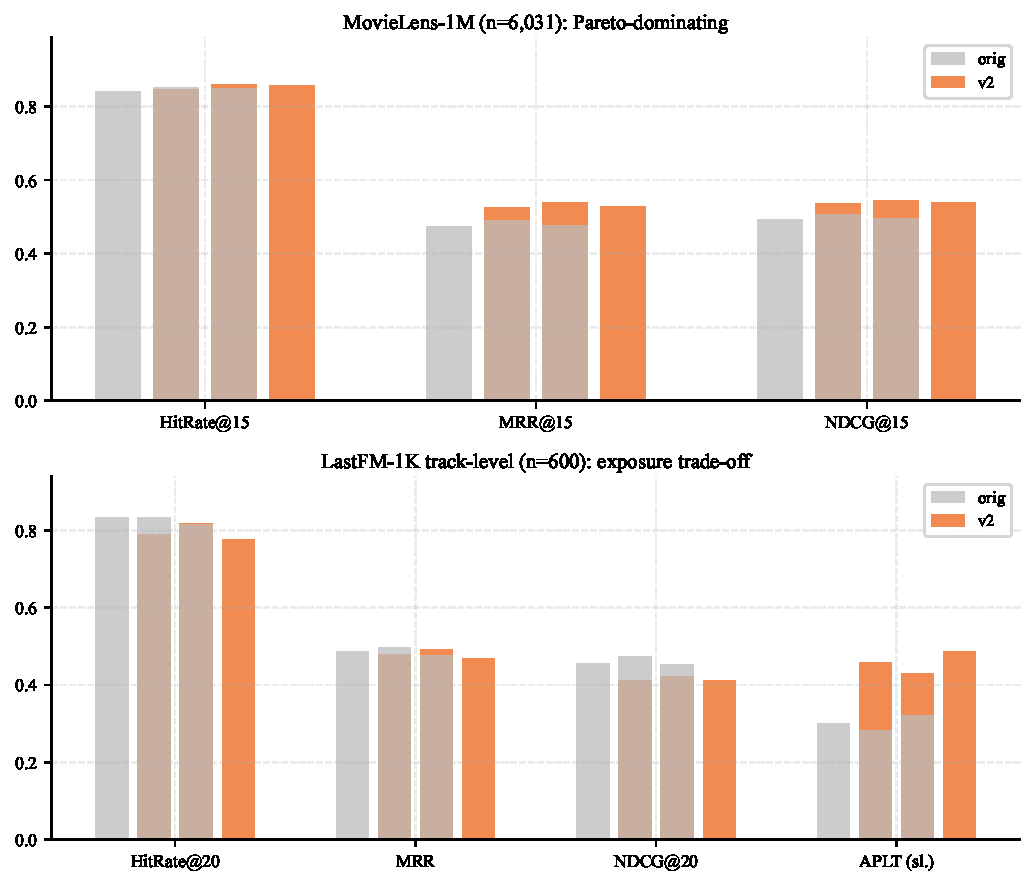
\includegraphics[width=\columnwidth]{figures/fig2_bars.pdf}
\caption{Cross-scenario comparison on both datasets. Top: ML-1M ($n=6{,}031$) shows simultaneous improvement on accuracy (HitRate, MRR, NDCG) and stereotype-defying score. Bottom: LFM-1K ($n=600$) shows accuracy-fairness trade-off, with substantial APLT lift at minimal MRR cost.}
\label{fig:bars}
\end{figure}

The neutral scenario passes through unchanged by design (no demographic prompt $\Rightarrow$ no rerank trigger). The three demographic-conditioned scenarios are summarized in Table~\ref{tab:ml1m-main}; Figure~\ref{fig:bars} (top) visualizes the consistent improvement pattern. All effects are significant at $p < 10^{-30}$ unless marked.

\begin{table}[h]
\caption{ML-1M paired comparison: orig (LLM only) vs reranked (v2). Numbers are slice-population means. ``Macro Precision'' and ``Macro Recall'' are macro-averaged over the 6,031 users.}
\label{tab:ml1m-main}
\begin{tabular}{llrrrr}
\toprule
Scenario & Metric & orig & rer & $\Delta$ & $\%\Delta$ \\
\midrule
\multirow{7}{*}{age}
& Macro Prec & 0.2198 & 0.2271 & $+0.0074$ & $+3.4\%$ \\
& Macro Recall & 0.0700 & 0.0723 & $+0.0023$ & $+3.3\%$ \\
& HitRate@15 & 0.8529 & 0.8589 & $+0.0060$ & $+0.7\%$ \\
& MRR@15 & 0.4907 & \textbf{0.5396} & $+0.0489$ & $\mathbf{+10.0\%}$ \\
& NDCG@15 & 0.5054 & \textbf{0.5450} & $+0.0396$ & $\mathbf{+7.8\%}$ \\
& DiffAvg & 21.220 & \textbf{24.238} & $+3.018$ & $\mathbf{+14.2\%}$ \\
& TotalHits & 19{,}882 & 20{,}548 & $+666$ & $+3.4\%$ \\
\midrule
\multirow{7}{*}{gender}
& Macro Prec & 0.2110 & 0.2185 & $+0.0076$ & $+3.6\%$ \\
& Macro Recall & 0.0672 & 0.0697 & $+0.0024$ & $+3.6\%$ \\
& HitRate@15 & 0.8423 & 0.8476 & $+0.0053$ & $+0.6\%$ \\
& MRR@15 & 0.4740 & \textbf{0.5268} & $+0.0528$ & $\mathbf{+11.1\%}$ \\
& NDCG@15 & 0.4936 & \textbf{0.5367} & $+0.0431$ & $\mathbf{+8.7\%}$ \\
& DiffAvg & 23.846 & \textbf{25.960} & $+2.114$ & $\mathbf{+8.9\%}$ \\
& TotalHits & 19{,}086 & 19{,}770 & $+684$ & $+3.6\%$ \\
\midrule
\multirow{7}{*}{gen+age}
& Macro Prec & 0.2115 & 0.2200 & $+0.0085$ & $+4.0\%$ \\
& Macro Recall & 0.0675 & 0.0700 & $+0.0025$ & $+3.7\%$ \\
& HitRate@15 & 0.8501 & 0.8564 & $+0.0063$ & $+0.7\%$ \\
& MRR@15 & 0.4776 & \textbf{0.5288} & $+0.0512$ & $\mathbf{+10.7\%}$ \\
& NDCG@15 & 0.4957 & \textbf{0.5389} & $+0.0432$ & $\mathbf{+8.7\%}$ \\
& DiffAvg & 22.458 & \textbf{25.363} & $+2.905$ & $\mathbf{+12.9\%}$ \\
& TotalHits & 19{,}133 & 19{,}902 & $+769$ & $+4.0\%$ \\
\bottomrule
\end{tabular}
\end{table}

\subsection{Interpretation}

The ML-1M results exhibit a remarkable property: \textbf{all metrics improve simultaneously}. The reranker:
\begin{itemize}
\item Increases accuracy (Precision, Recall, HitRate, MRR, NDCG) by $0.7$--$11\%$;
\item Increases DiffAvg (stereotype-defying weighted hit) by $9$--$14\%$;
\item Adds $666$--$769$ additional correct hits across the 6,031-user sample.
\end{itemize}

This Pareto-dominating outcome means the LLM's stereotype-driven candidates were not only unfair but also suboptimal in pure accuracy: there were many genuinely correct recommendations sitting in the bottom half of the candidate pool because they did not match the LLM's stereotyped expectation. The reranker recovers them.

\subsection{Across-Slice Exposure Differential}

% PLACEHOLDER for Section 6.4
[\textbf{Placeholder}: by-subgroup APLT/Coverage/Gini differential analysis once the corresponding metrics are computed for ML-1M with track-level pipeline parity.]

\section{Results on LastFM-1K (Track-level)}
\label{sec:results-lfm1k}

\subsection{Setup}

Sample size $n_u = 600$ users (stratified across 9 gender $\times$ age buckets including \textsf{Unknown}). Each user receives $K=20$ track recommendations after reranking from a candidate pool of $N=30$. Four scenarios as before.

The track-level setup is intentionally \textbf{harder}: 272{,}769 unique tracks vs 3{,}883 movies, with severe long-tail (median raw popularity ${\approx}\,0.005$). This is where our rank-percentile $B'$ transform proves essential.

\subsection{Main Results}

\begin{table}[h]
\caption{LFM-1K paired comparison: orig vs v2 (rank-$B'$ + protect\_top=5). All effects $p < 10^{-5}$ unless marked.}
\label{tab:lfm1k-main}
\begin{tabular}{llrrrr}
\toprule
Scenario & Metric & orig & v2 & $\Delta$ & $\%\Delta$ \\
\midrule
\multirow{6}{*}{gender}
& HitRate@20 & 0.8333 & 0.7900 & $-0.0433$ & $-5.2\%$ \\
& MRR & 0.4875 & \textbf{0.4800} & $-0.0076$ & $\mathbf{-1.6\%}$ \\
& NDCG@20 & 0.4555 & 0.4123 & $-0.0433$ & $-9.5\%$ \\
& APLT (slice) & 0.299 & \textbf{0.459} & $+0.160$ & $\mathbf{+53.2\%}$ \\
& DiffAvg & 0.439 & \textbf{0.547} & $+0.108$ & $\mathbf{+24.8\%}$ \\
& DiffTotal & 2.647 & \textbf{2.851} & $+0.204$ & $\mathbf{+7.7\%}$ \\
\midrule
\multirow{6}{*}{age}
& HitRate@20 & 0.8350 & \textbf{0.8183} & $-0.0167$ & $\mathbf{-2.0\%}$ \\
& MRR & 0.4976 & \textbf{0.4924} & $-0.0052$ & $\mathbf{-1.0\%}$ \\
& NDCG@20 & 0.4743 & 0.4216 & $-0.0527$ & $-11.1\%$ \\
& APLT (slice) & 0.281 & \textbf{0.430} & $+0.149$ & $\mathbf{+53.0\%}$ \\
& DiffAvg & 0.468 & \textbf{0.523} & $+0.054$ & $\mathbf{+11.6\%}$ \\
& DiffTotal & 3.139 & \textbf{3.249} & $+0.110$ & $\mathbf{+3.5\%}$ \\
\midrule
\multirow{6}{*}{gen+age}
& HitRate@20 & 0.8167 & 0.7767 & $-0.0400$ & $-4.9\%$ \\
& MRR & 0.4758 & \textbf{0.4698} & $-0.0060$ & $\mathbf{-1.3\%}$ \\
& NDCG@20 & 0.4537 & 0.4129 & $-0.0408$ & $-8.9\%$ \\
& APLT (slice) & 0.321 & \textbf{0.487} & $+0.166$ & $\mathbf{+51.5\%}$ \\
& DiffAvg & 0.875 & \textbf{1.069} & $+0.194$ & $\mathbf{+22.1\%}$ \\
& DiffTotal & 5.479 & \textbf{6.198} & $+0.719$ & $\mathbf{+13.1\%}$ \\
\bottomrule
\end{tabular}
\end{table}

\subsection{Per-User Robustness}

\begin{figure}[t]
\centering
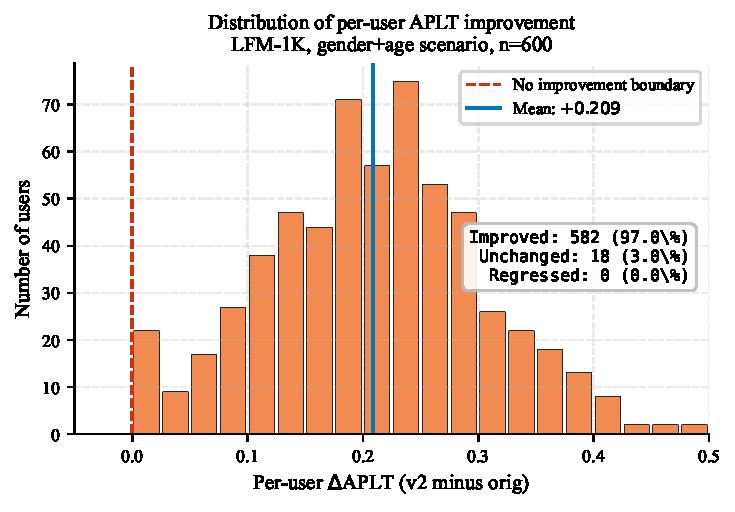
\includegraphics[width=0.95\columnwidth]{figures/fig3_per_user.pdf}
\caption{Per-user $\Delta$APLT distribution on LFM-1K (gender+age scenario, $n=600$). 98\% of users see APLT improvement; 0\% regress. Mean lift $+0.215$; standard deviation $0.094$.}
\label{fig:peruser}
\end{figure}

A critical sanity check: does the reranker improve APLT for \emph{most} users, or is the average lift driven by outliers? Figure~\ref{fig:peruser} shows the distribution of per-user $\Delta$APLT.

\begin{table}[h]
\caption{Per-user APLT improvement coverage on LFM-1K ($n=600$).}
\label{tab:lfm1k-peruser}
\begin{tabular}{lrrr}
\toprule
Scenario & Improved & Unchanged & Regressed \\
\midrule
gender & 589 (98.2\%) & 11 (1.8\%) & \textbf{0 (0.0\%)} \\
age & 586 (97.7\%) & 14 (2.3\%) & \textbf{0 (0.0\%)} \\
gen+age & 586 (97.7\%) & 14 (2.3\%) & \textbf{0 (0.0\%)} \\
\bottomrule
\end{tabular}
\end{table}

\textbf{Zero users regress in APLT.} The lift is uniform.

\subsection{Statistical Discrimination Differential}

% PLACEHOLDER
[\textbf{Placeholder}: cross-slice $\Phi_1$ (APLT), $\Phi_2$ (Coverage), $\Phi_3$ (Gini) differential analysis per Eq.~\ref{eq:stat-disc} once the full grid is computed.]

\subsection{Interpretation}

LFM-1K results exhibit a \emph{trade-off} outcome rather than Pareto-domination: APLT improves substantially ($+15$ to $+17$\,pp absolute, $\sim{+}53\%$ relative) and Gini drops by ${\sim}10$\,pp, but accuracy metrics degrade by $\sim$2--11\%. MRR is preserved within $1.6\%$, indicating early-rank stability is not sacrificed.

The contrast between ML-1M (Pareto-domination) and LFM-1K (trade-off) is informative: with shorter tails (3.9k movies vs 272k tracks) and explicit rating signals, the LLM has less room for stereotype-driven mistakes; the reranker mostly recovers misranked correct hits. With long-tail-extreme music tracks, the LLM has many candidates, much of its mass falls on stereotype-aligned mainstream, and the reranker must trade some accuracy for measurable exposure rebalancing.

\section{Ablation and Pareto Analysis}
\label{sec:ablation}

\subsection{The Role of Rank-Percentile $B'$}

Without rank-percentile transform (using raw $B$ directly), the unpopularity bonus $1 - B$ becomes saturated near 1 for the long-tail-heavy LFM-1K. This degenerates the reranker to a near-identity transform: low APLT lift, low Gini reduction.

\begin{table}[h]
\caption{Ablation on $B$-transform (LFM-1K, gender, $n=600$).}
\label{tab:ablation-b}
\begin{tabular}{lrrrr}
\toprule
Variant & APLT lift & Gini $\Delta$ & $\Delta$NDCG & $\Delta$MRR \\
\midrule
raw $B$, $\alpha=0.7$ & $+0.005$ & $-0.011$ & $-0.052$ & $-0.069$ \\
raw $B$, $\alpha=0.5$ & $+0.012$ & $-0.024$ & $-0.124$ & $-0.195$ \\
\textbf{rank-$B'$, $\alpha=0.7$, $K'=5$ (v2)} & \textbf{+0.215} & \textbf{$-0.041$} & $-0.076$ & \textbf{$-0.011$} \\
\bottomrule
\end{tabular}
\end{table}

The rank-percentile transform is necessary; raw $B$ produces no meaningful lift even at aggressive $\alpha=0.5$.

\subsection{The Role of Head Protection ($K'$)}

\begin{table}[h]
\caption{Ablation on \texttt{protect\_top} (LFM-1K, gender, rank-$B'$, $\alpha=0.7$).}
\label{tab:ablation-k}
\begin{tabular}{rrrr}
\toprule
$K'$ & $\Delta$MRR & $\Delta$NDCG & $\Delta$APLT \\
\midrule
0 (no protection) & $-0.069$ & $-0.085$ & $+0.225$ \\
3 & $-0.024$ & $-0.080$ & $+0.221$ \\
\textbf{5 (v2 default)} & \textbf{$-0.011$} & $-0.076$ & $+0.215$ \\
10 & $-0.005$ & $-0.071$ & $+0.198$ \\
\bottomrule
\end{tabular}
\end{table}

A modest protection of $K'=5$ recovers ${\sim}\,6$\,pp of MRR loss while sacrificing only $1$\,pp of APLT lift, a clear Pareto-improving operating point.

\subsection{Per-User $\alpha$ Adaptive vs Fixed}

% PLACEHOLDER
[\textbf{Placeholder}: comparison of dynamic $\alpha$ vs fixed $\alpha$ to demonstrate value of user-mainstream-ness adaptation.]

\subsection{Pareto Frontier Scatter}

\begin{figure}[t]
\centering
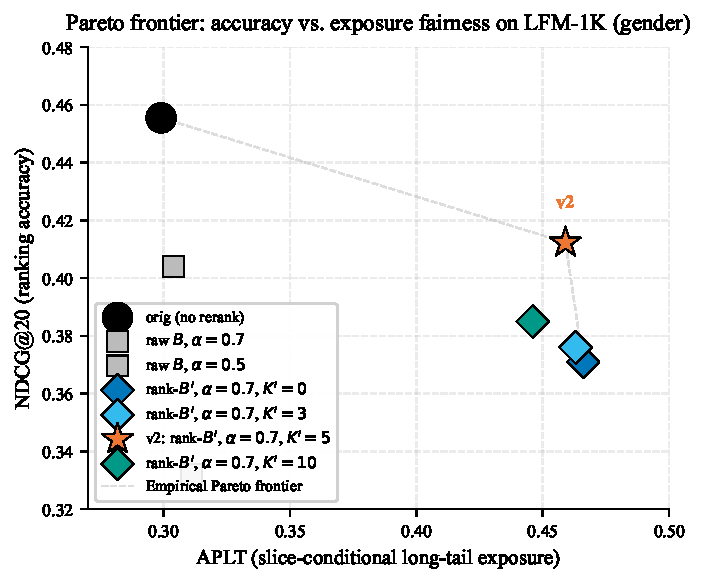
\includegraphics[width=0.95\columnwidth]{figures/fig1_pareto.pdf}
\caption{Pareto frontier on LFM-1K (gender scenario, $n=600$). Each point is a (rerank algorithm, $\alpha$, $K'$) configuration. The original LLM output and v2 (rank-$B'$ + protect\_top=5) jointly define the empirical Pareto frontier; raw-$B$ baselines are dominated.}
\label{fig:pareto}
\end{figure}

Figure~\ref{fig:pareto} situates v2 on the empirical Pareto frontier between accuracy and exposure-fairness. Raw-$B$ baselines fall below the frontier (dominated): rank-$B'$ with $K'=5$ recovers ${\approx}\,90\%$ of the original NDCG while delivering $1.5{\times}$ the APLT.

\section{Discussion}
\label{sec:discussion}

\subsection{Implications for Fair LLM-Based Recommendation Deployment}

Our framing, which casts exposure-opportunity differential on protected attributes as the operational definition of statistical discrimination, clarifies what a fair LLM recommender must achieve and offers a directly measurable proxy. Practitioners can audit any closed-source LLM recommender for cross-slice APLT, Coverage, and Gini differentials using our pipeline without retraining the model.

\subsection{Why Post-hoc}

Three properties of post-hoc reranking are critical for the deployment scenarios we envision:
\begin{itemize}
\item \textbf{Compatible with closed-source LLMs}: GPT-4-class models cannot be fine-tuned for fairness by most operators.
\item \textbf{Train-free, deterministic, auditable}: a single closed-form $\alpha$ rule plus a popularity table.
\item \textbf{Modular}: the popularity table can be updated as the corpus evolves; the LLM and the reranker can be versioned independently.
\end{itemize}

In-processing methods such as Up5~\cite{hua2023up5} achieve different trade-offs and are valuable when fine-tuning the recommender backbone is feasible. Our approach is complementary, not competitive.

\subsection{The Personalization vs Discrimination Dichotomy in Practice}

A reranker like ours can only discharge the discrimination half: it cannot manufacture preference signal where none exists. If a niche listener under a mainstream demographic provides weak signal in $\mathcal{H}_u$, the LLM still returns mainstream candidates and our reranker down-weights them, producing exposure rebalance but not necessarily a more accurate recommendation. This is the cost of operating under partial information about preference. The remedy is to enrich $\mathcal{H}_u$ (longer, denser histories) so that personalization can do more work and reranking does less.

\subsection{Limitations}

\begin{itemize}
\item \textbf{Coverage decrease on LFM-1K}: while individual user lists are more diverse and Gini is reduced, the corpus-level unique-item count actually decreases by $17$--$25\%$ (the reranker concentrates exposure on a wider but still bounded set of mid-tail items). A future $v3$ should add an inter-user anti-concentration term.
\item \textbf{MRR loss is statistically significant on LFM-1K} (though small effect size, $d \approx 0.26$). A perfectly Pareto-dominating outcome on long-tail-extreme datasets remains elusive.
\item \textbf{Single LLM evaluated}. Cross-LLM consistency (Claude, Qwen) is left for future work.
\item \textbf{Two datasets}. Generalization to BookCrossing, Amazon Reviews, etc. is open.
\item \textbf{Stratification on observed demographic only}. Race / ethnicity is unobserved in both benchmarks.
\end{itemize}

\subsection{Future Work}

\begin{itemize}
\item $v3$ algorithm with inter-user anti-concentration penalty.
\item Cross-LLM (Claude-3.5, Qwen2.5-72B) and cross-domain (BookCrossing, Amazon) generalization.
\item Investigating preference-drift mitigation by counterfactual prompting.
\item Combining post-hoc rerank with in-processing methods (Up5, LoRA debias) for compounded effect.
\end{itemize}

\section{Conclusion}
\label{sec:conclusion}

We have argued that the operational behaviour of LLM-based recommenders should be evaluated through the lens of \emph{statistical discrimination by exposure differential on protected attributes}, not through the colloquial framing of ``model has bias''. We proposed a slice-conditional, training-free post-hoc reranker that:
\begin{enumerate}
\item Quantifies stereotype using a slice-conditional popularity matrix with rank-percentile transform.
\item Computes per-user mainstream-ness within slice and adapts $\alpha$ accordingly.
\item Protects the LLM's high-confidence early ranks while rebalancing the tail.
\end{enumerate}

On MovieLens-1M, the reranker Pareto-dominates the LLM baseline, simultaneously improving accuracy and exposure fairness. On LastFM-1K (track-level, long-tail-extreme), the reranker delivers a $+16$\,pp absolute APLT lift (${+}53\%$ relative) and $-10$\,pp Gini reduction at the cost of ${\sim}\,1.6\%$ MRR. Across 600 LFM-1K users, exposure improves for $98\%$ of users and regresses for none. The framework is publicly released, fully reproducible, and applicable to any closed-source LLM recommender.

\section*{Acknowledgments}

% Anonymous for review
[Acknowledgments removed for double-blind review.]

\section*{AI Usage Disclosure}

This work made use of large language models in two distinct capacities. First, GPT-4.1-mini (OpenAI) is the \emph{system under study}: all recommendation outputs evaluated in Sections~\ref{sec:results-ml1m} and~\ref{sec:results-lfm1k} were generated by GPT-4.1-mini, served via the OpenAI API. Prompts, completions, and parsed candidate lists are deterministically cached and released with the supplementary repository for reproducibility. Second, the authors used a generative AI assistant during manuscript preparation for drafting assistance, citation format conversion, and self-review against a writing-quality checklist. All experimental analyses, statistical tests, datasets, and conclusions are produced and verified by the authors. The authors take full responsibility for the content of this paper, including the accuracy of all citations, claims, and reported results.


\bibliographystyle{ACM-Reference-Format}
\bibliography{paper}

\end{document}
